\documentclass[tikz,border=10pt]{standalone}
\begin{document}
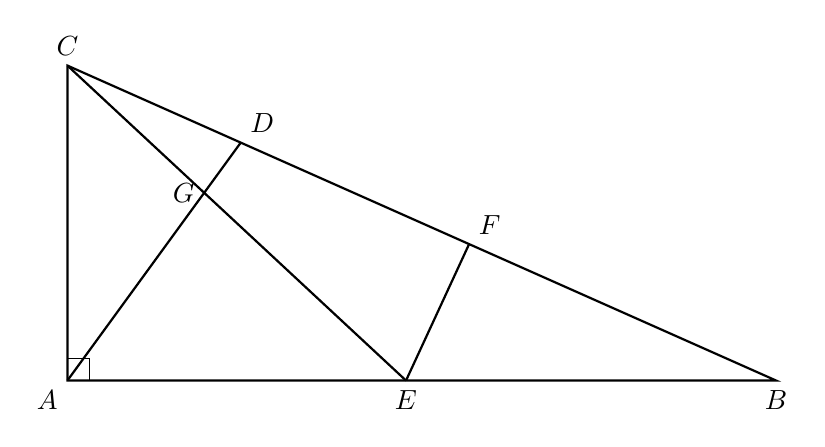
\begin{tikzpicture}[scale=1]
  \coordinate (A) at (0,0);
  \coordinate (B) at (9,0);
  \coordinate (C) at (0,4);
  \coordinate (E) at (4.3,0);
  \coordinate (D) at (2.2,3.02);
  \coordinate (F) at (5.1,1.73);
  \coordinate (G) at (1.74,2.38);

  \draw[thick] (A) -- (B) -- (C) -- cycle;
  \draw[thick] (A) -- (D);
  \draw[thick] (C) -- (E);
  \draw[thick] (E) -- (F);

  % right-angle mark at A
  \draw (0.28,0) -- (0.28,0.28) -- (0,0.28);

  \node[above] at (C) {$C$};
  \node[above right] at (D) {$D$};
  \node[above right] at (F) {$F$};
  \node[left] at (G) {$G$};
  \node[below left] at (A) {$A$};
  \node[below] at (E) {$E$};
  \node[below] at (B) {$B$};
\end{tikzpicture}
\end{document}
